\documentclass[tikz,border=4pt]{standalone}

\usepackage{amsmath}
\usepackage{xcolor}

\definecolor{exactblue}{HTML}{0000FF}

\begin{document}

% iii-ii-l
% MRM special fibre for [III-II_l]

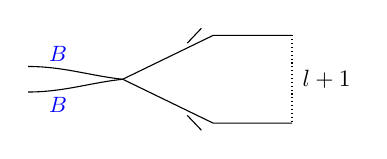
\begin{tikzpicture}[xscale=1,yscale=0.9]

% Type III tangency on the left
\draw
  (-1.2,0.18)
  .. controls (-0.75,0.18) and (-0.42,0.05) ..
  (0,0);

\draw
  (-1.2,-0.18)
  .. controls (-0.75,-0.18) and (-0.42,-0.05) ..
  (0,0);

% The two branches open out to form the loop
\draw
  (0,0) -- (1.15,0.62) -- (2.15,0.62);

\draw
  (0,0) -- (1.15,-0.62) -- (2.15,-0.62);

% Schematic continuation of the loop
\draw[densely dotted]
  (2.15,0.62) -- (2.15,-0.62);

% Small transverse marks
\draw
  (0.82,0.51) -- (1.00,0.72);

\draw
  (0.82,-0.51) -- (1.00,-0.72);

% Labels on the two branches of the type III part
\node[text=exactblue,scale=0.8]
  at (-0.82,0.36) {$B$};

\node[text=exactblue,scale=0.8]
  at (-0.82,-0.36) {$B$};

% Parameterised part of the loop
\node[scale=0.85,right]
  at (2.18,0) {$l+1$};

\end{tikzpicture}

\end{document}
